\documentclass{ximera}

%% You can put user macros here
%% However, you cannot make new environments

\listfiles

\graphicspath{{./}{firstExample/}{secondExample/}}

\usepackage{tikz}
\usepackage{tkz-euclide}
\usepackage{tikz-3dplot}
\usepackage{tikz-cd}
\usetikzlibrary{shapes.geometric}
\usetikzlibrary{arrows}
\usetikzlibrary{decorations.pathmorphing,patterns}
\usetkzobj{all}
\pgfplotsset{compat=1.13} % prevents compile error.

\renewcommand{\vec}[1]{\mathbf{#1}}
\newcommand{\RR}{\mathbb{R}}
\newcommand{\dfn}{\textit}
\newcommand{\dotp}{\cdot}
\newcommand{\id}{\text{id}}
\newcommand\norm[1]{\left\lVert#1\right\rVert}
 
\newtheorem{general}{Generalization}
\newtheorem{initprob}{Exploration Problem}

\tikzstyle geometryDiagrams=[ultra thick,color=blue!50!black]

\usepackage{mathtools}

\title{2.6 Integrating Factors}


\begin{document}

\begin{abstract}
We show how multiplying an equation by an integrating factor can make the equation exact, and we give examples where this is a nice technique for solving a first-order equation.
\end{abstract}

\maketitle



\section*{Integrating Factors}
In \href{https://ximera.osu.edu/ode/main/exactEquations/exactEquations}{Trench 2.5}, Exact Equations, we saw that if $M$, $N$, $M_y$ and $N_x$ are
continuous and $M_y=N_x$ on an open rectangle $R$ then
\begin{equation} \label{eq:2.6.1}
M(x,y)\,dx+N(x,y)\,dy=0
\end{equation}
is exact on $R$. Sometimes an equation that isn't  exact can be made
exact by multiplying it by an appropriate function. For example,
\begin{equation}\label{eq:2.6.2}
(3x+2y^2)\,dx+2xy\,dy=0
\end{equation}
is  not exact, since
$M_y(x,y)=4y\neq  N_x(x,y)=2y$ in \eqref{eq:2.6.2}.
 However, multiplying \eqref{eq:2.6.2}  by $x$ yields
\begin{equation}\label{eq:2.6.3}
(3x^2+2xy^2)\,dx+2x^2y\,dy=0,
\end{equation}
which is exact, since
$M_y(x,y)=N_x(x,y)=4xy$ in \eqref{eq:2.6.3}.
Solving \eqref{eq:2.6.3} by Procedure \ref{proc:solvingExactEq} of \href{https://ximera.osu.edu/ode/main/exactEquations/exactEquations}{Trench 2.5},
 yields the implicit solution
$$
x^3+x^2y^2=c.
$$

A function $\mu=\mu(x,y)$ is  an \dfn{integrating factor} for
\eqref{eq:2.6.1}  if
\begin{equation}\label{eq:2.6.4}
 \mu(x,y)M (x,y)\,dx+\mu(x,y)N (x,y)\,dy=0
 \end{equation}
 is exact. If we know an integrating
factor $\mu$ for \eqref{eq:2.6.1}, we can solve the exact equation
\eqref{eq:2.6.4} by Procedure \ref{proc:solvingExactEq} \href{https://ximera.osu.edu/ode/main/exactEquations/exactEquations}{Trench 2.5}. It would be
nice
if we could say that \eqref{eq:2.6.1} and \eqref{eq:2.6.4} always have the
same solutions, but this isn't so. For example, a solution
$y=y(x)$ of \eqref{eq:2.6.4} such that $\mu(x,y(x))=0$ on some interval
$a<x<b$ could fail to be a solution of \eqref{eq:2.6.1}
%(Exercise~\ref{exer:2.6.1})
, while
\eqref{eq:2.6.1} may have a solution $y=y(x)$ such that $\mu(x,y(x)) $
isn't even defined 
%(Exercise~\ref{exer:2.6.2})
. Similar comments
apply if $y$ is the independent variable and $x$ is the dependent
variable  in \eqref{eq:2.6.1} and \eqref{eq:2.6.4}.  However, if $\mu(x,y)$
is defined and nonzero for all $(x,y)$,  \eqref{eq:2.6.1}  and
\eqref{eq:2.6.4} are equivalent; that is, they have the same solutions.

\subsection*{Finding Integrating Factors}

By applying Theorem~\ref{thmtype:2.5.2} (with $M$ and $N$ replaced by $\mu M$
and $\mu N$), we see that \eqref{eq:2.6.4} is exact on an open rectangle
$R$ if $\mu M$, $\mu N$, $(\mu M)_y$, and $(\mu N)_x$ are continuous
and
$$
\frac{\partial}{\partial y}(\mu M)=\frac{\partial}{\partial x}
(\mu N) \quad\text{or, equivalently,}\quad
\mu_yM+\mu M_y=\mu_xN+\mu N_x
$$
on $R$. It's better to rewrite the last equation as
\begin{equation} \label{eq:2.6.5}
\mu(M_y-N_x)=\mu_xN-\mu_yM,
\end{equation}
which  reduces to  the known result for exact equations;
that is, if $M_y=N_x$ then \eqref{eq:2.6.5} holds with $\mu=1$, so
\eqref{eq:2.6.1} is exact.

You may think  \eqref{eq:2.6.5} is of little value, since it involves
\textit{partial} derivatives of the unknown integrating factor $\mu$,
and we haven't studied methods for solving such equations. However,
we'll now show that \eqref{eq:2.6.5} is useful if we restrict our search
to integrating factors that are products of a function of
$x$ and a function of $y$; that is,
$\mu(x,y)=P(x)Q(y)$.
We're not saying that \textit{every} equation
 $M\,dx+N\,dy=0$ has an integrating factor of this
form;   rather, we're saying that \textit{some} equations have
such integrating
factors.  We'll now develop a way to determine whether a given
equation has such an integrating factor, and a method for finding the
integrating factor in this case.


If $\mu(x,y)=P(x)Q(y)$, then $\mu_x(x,y)=P'(x)Q(y)$ and
$\mu_y(x,y)=P(x)Q'(y)$, so \eqref{eq:2.6.5} becomes
\begin{equation} \label{eq:2.6.6}
P(x)Q(y)(M_y-N_x)=P'(x)Q(y)N-P(x)Q'(y)M,
\end{equation}
or, after dividing through by $P(x)Q(y)$,
\begin{equation} \label{eq:2.6.7}
M_y-N_x=\frac{P'(x)}{P(x)}N-\frac{Q'(y)}{Q(y)}M.
\end{equation}
Now let
$$
p(x)=\frac{P'(x)}{P(x)}\quad \text{and}\quad q(y)=\frac{Q'(y)}{Q(y)},
$$
so \eqref{eq:2.6.7} becomes
\begin{equation} \label{eq:2.6.8}
M_y-N_x=p(x)N-q(y)M.
\end{equation}

We obtained \eqref{eq:2.6.8} by \textit{assuming} that $M\,dx+N\,dy=0$ has
an integrating factor $\mu(x,y)=P(x)Q(y)$. However, we can
now view \eqref{eq:2.6.7} differently: If there are functions $p=p(x)$
and $q=q(y)$  that satisfy \eqref{eq:2.6.8} and we define
\begin{equation} \label{eq:2.6.9}
P(x)=\pm e^{\int p(x)\,dx}\quad\text{and}\quad
Q(y)=\pm e^{\int q(y)\,dy},
\end{equation}
then reversing the steps that led from \eqref{eq:2.6.6} to
\eqref{eq:2.6.8} shows that $\mu(x,y)=P(x)Q(y)$ is an integrating factor
for $M\,dx+N\,dy=0$. In using this result, we take the constants of
integration in \eqref{eq:2.6.9} to be zero and choose the signs
conveniently so the integrating factor has the simplest form.

There's no simple general method for ascertaining
whether functions $p=p(x)$ and $q=q(y)$ satisfying \eqref{eq:2.6.8}
exist. However, the next theorem gives simple sufficient
conditions for the given equation to have an integrating factor that
depends on only one of the independent variables $x$ and $y$, and for
finding an integrating factor in this case.

\begin{theorem}\label{thmtype:2.6.1}
Let $M,$ $N,$ $M_y,$ and $N_x$ be continuous on an open rectangle $R.$
Then:
\begin{enumerate}
\item \label{item:2.6.1a} % (a)
 If $(M_y-N_x)/N$ is independent
of $y$ on $R$ and  we define
$$
p(x)=\frac{M_y-N_x}{N}
$$
 then
\begin{equation}\label{eq:2.6.10}
\mu(x)=\pm e^{\int p(x)\,dx}
\end{equation}
is an integrating factor for
\begin{equation}\label{eq:2.6.11}
M(x,y)\,dx+N(x,y)\,dy=0
\end{equation}
on $R.$
\item \label{item:2.6.1b} % (b)
If $(N_x-M_y)/M$ is independent of $x$ on
$R$ and we define
$$
q(y)=\frac{N_x-M_y}{M},
$$
then
\begin{equation}\label{eq:2.6.12}
\mu(y)=\pm e^{\int q(y)\,dy}
\end{equation}
 is an integrating factor for \eqref{eq:2.6.11} on $R.$
\end{enumerate}
\end{theorem}



\begin{proof} \ref{item:2.6.1a}
If $(M_y-N_x)/N$ is independent of $y$, then \eqref{eq:2.6.8}
 holds with $p=(M_y-N_x)/N$ and $q\equiv0$. Therefore
 $$
P(x)=\pm e^{\int p(x)\,dx}\quad\text{and}\quad Q(y)=\pm e^{\int
q(y)\,dy}=\pm e^0=\pm1,
 $$
so \eqref{eq:2.6.10} is an integrating factor for \eqref{eq:2.6.11} on $R$.

\ref{item:2.6.1b} If $(N_x-M_y)/M$ is independent of $x$ then eqref{eq:2.6.8} holds
with $p\equiv0$ and $q=(N_x-M_y)/M$, and a similar argument shows that
\eqref{eq:2.6.12} is an integrating factor for \eqref{eq:2.6.11} on $R$.
\end{proof}

The next two examples show how to apply
Theorem~\ref{thmtype:2.6.1}.

\begin{example}\label{example:2.6.1}
Find an integrating factor for the equation
\begin{equation}\label{eq:2.6.13}
(2xy^3-2x^3y^3-4xy^2+2x)\,dx+(3x^2y^2+4y)\,dy=0
\end{equation}
and solve the equation.
\begin{explanation}
In \eqref{eq:2.6.13}
$$
M=2xy^3-2x^3y^3-4xy^2+2x,\ N=3x^2y^2+4y,
$$
and
$$
M_y-N_x=(6xy^2-6x^3y^2-8xy)-6xy^2=-6x^3y^2-8xy,
$$
so \eqref{eq:2.6.13}  isn't  exact. However,
$$
\frac{M_y-N_x}{N}=-\frac{6x^3y^2+8xy}{3x^2y^2+4y}=-2x
$$
is independent of $y$, so Theorem~\ref{thmtype:2.6.1}\ref{item:2.6.1b} applies
with
$p(x)=-2x$. Since
$$
\int p (x)\,dx=-\int 2x\,dx=-x^2,
$$
 $\mu(x)=e^{-x^2}$ is an
integrating factor.  Multiplying \eqref{eq:2.6.13} by $\mu$ yields the
exact equation
\begin{equation}\label{eq:2.6.14}
e^{-x^2}(2xy^3-2x^3y^3-4xy^2+2x)\,dx+
 e^{-x^2}(3x^2y^2+4y)\,dy=0.
\end{equation}

To solve this equation, we must find a
function $F$ such that
\begin{equation}\label{eq:2.6.15}
F_x(x,y)=e^{-x^2}(2xy^3-2x^3y^3-4xy^2+2x)
\end{equation}
 and
\begin{equation}\label{eq:2.6.16}
F_y(x,y)=e^{-x^2}(3x^2y^2+4y).
\end{equation}
 Integrating \eqref{eq:2.6.16} with respect to $y$ yields
\begin{equation}\label{eq:2.6.17}
F(x,y)=e^{-x^2}(x^2y^3+2y^2)+\psi(x).
\end{equation}
 Differentiating this with respect to $x$ yields
$$
F_x(x,y)=e^{-x^2}(2xy^3-2x^3y^3-4xy^2)+\psi'(x).
$$
Comparing this with \eqref{eq:2.6.15} shows that $\psi'(x)=
2xe^{-x^2}$;  therefore, we can let $\psi(x)=-e^{-x^2}$ in
\eqref{eq:2.6.17} and conclude that
$$
e^{-x^2}\left(y^2(x^2y+2)-1\right)=c
$$
is an implicit solution of \eqref{eq:2.6.14}. It is also an implicit solution
of \eqref{eq:2.6.13}.

The figure below  shows a  direction field and some integral curves
for \eqref{eq:2.6.13}

\begin{image}
 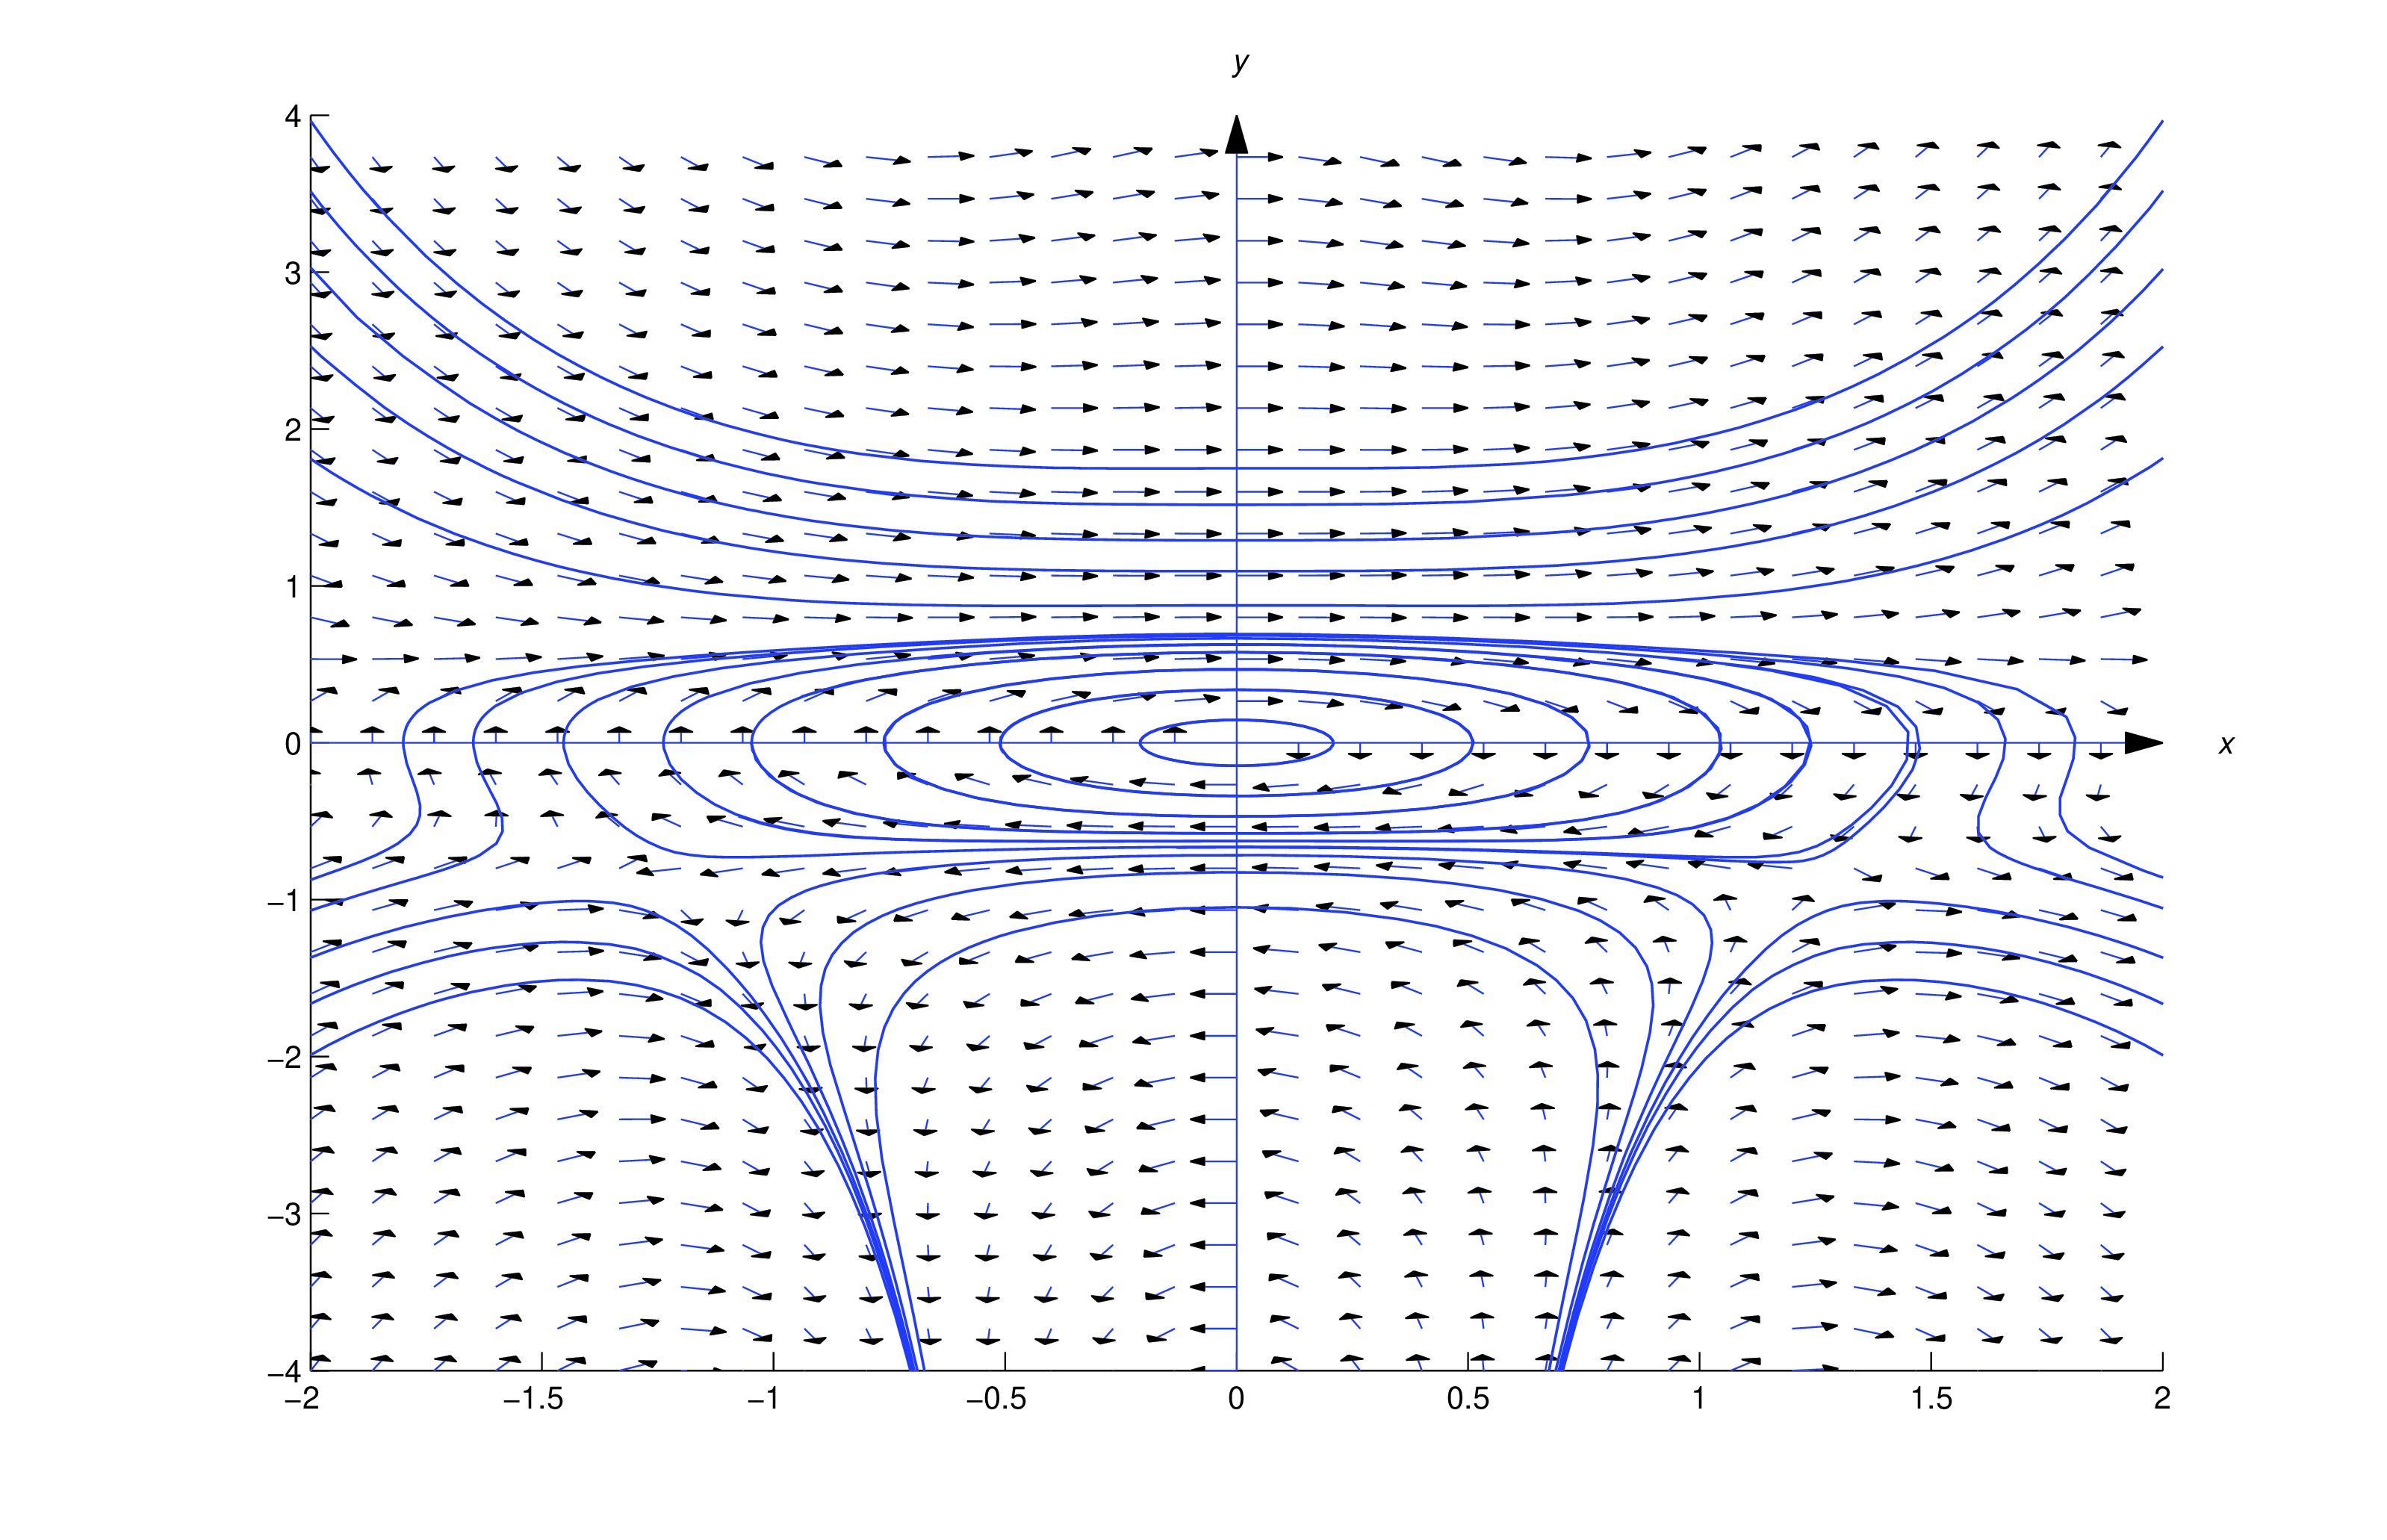
\includegraphics[height=1.5in]{fig020601.jpg}
\end{image}

\end{explanation}
\end{example}


\begin{example}\label{example:2.6.2}
Find an integrating factor for
\begin{equation}\label{eq:2.6.18}
2xy^3\,dx+(3x^2y^2+x^2y^3+1)\,dy=0
\end{equation}
and solve the equation.

\begin{explanation} In \eqref{eq:2.6.18},
$$
M=2xy^3,\quad N=3x^2y^2+x^2y^3+1,
$$
and
$$
M_y-N_x=6xy^2-(6xy^2+2xy^3)=-2xy^3,
$$
so \eqref{eq:2.6.18} isn't  exact.  Moreover,
$$
\frac{M_y-N_x}{N}=-\frac{2xy^3}{3x^2y^2+x^2y^2+1}
$$
is not independent of $y$, so Theorem~\ref{thmtype:2.6.1}\ref{item:2.6.1a} does not
apply. However,   Theorem~\ref{thmtype:2.6.1}\ref{item:2.6.1b} does apply, since
$$
\frac{N_x-M_y}{M}=\frac{2xy^3}{2xy^3}=1
$$
is independent of $x$, so we can take $q(y)=1$.
 Since
$$
\int q(y)\,dy=\int\,dy=y,
$$
  $\mu(y)=e^y$ is
an integrating factor. Multiplying \eqref{eq:2.6.18} by $\mu$ yields the
exact equation
\begin{equation}\label{eq:2.6.19}
2xy^3e^y\,dx+(3x^2y^2+x^2y^3+1)e^y\,dy=0.
\end{equation}
To solve this equation, we must find a
function $F$ such that
\begin{equation}\label{eq:2.6.20}
F_x(x,y)=2xy^3e^y
\end{equation}
 and
\begin{equation}\label{eq:2.6.21}
F_y(x,y)=(3x^2y^2+x^2y^3+1)e^y.
\end{equation}
 Integrating \eqref{eq:2.6.20} with respect to $x$ yields
\begin{equation}\label{eq:2.6.22}
F(x,y)=x^2y^3e^y+\phi(y).
\end{equation}
Differentiating this with respect to $y$ yields
$$
F_y=(3x^2y^2+x^2y^3)e^y+\phi'(y),
$$
and comparing this with \eqref{eq:2.6.21} shows that $\phi'(y)=e^y$.
 Therefore we set $\phi(y)=e^y$ in \eqref{eq:2.6.22} and conclude
that
$$
(x^2y^3+\answer{1})e^y=c
$$
is an implicit solution of \eqref{eq:2.6.19}.
It is also an implicit solution
 of \eqref{eq:2.6.18}. The figure below shows a direction
field and some integral curves for \eqref{eq:2.6.18}.
\begin{image}
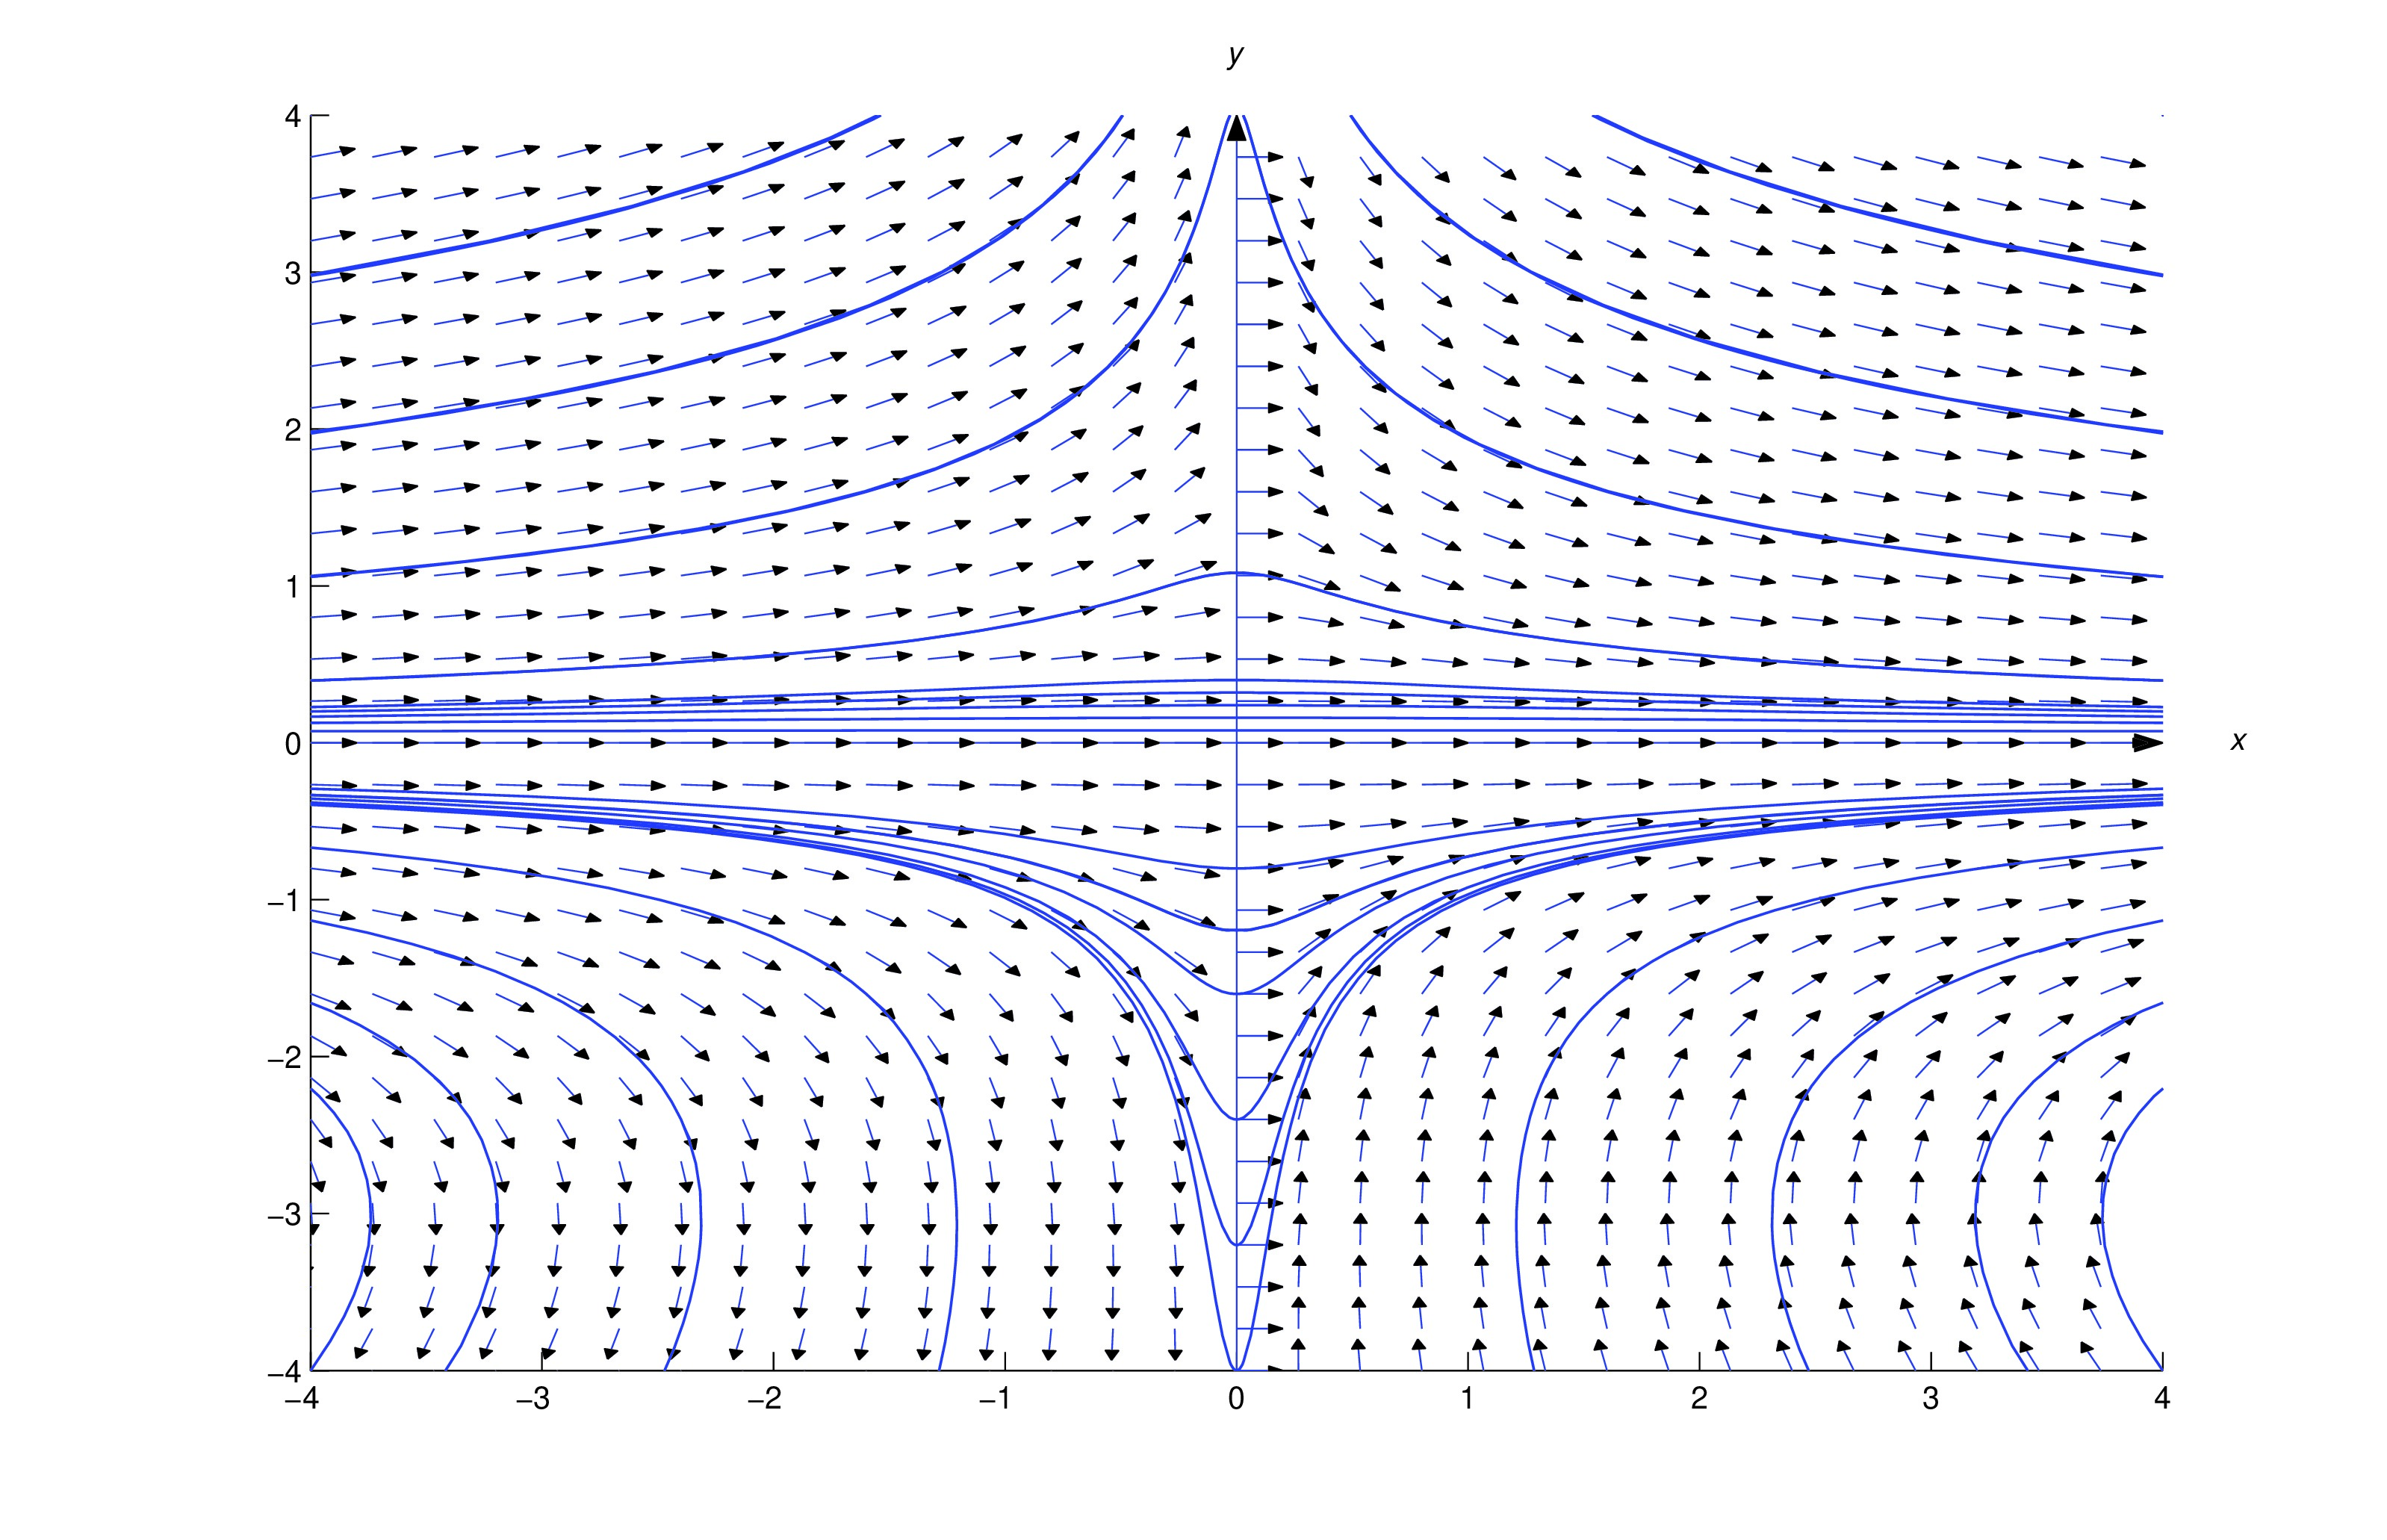
\includegraphics[height=1.5in]{fig020602.jpg}
\end{image}

\end{explanation}
\end{example}

Theorem~\ref{thmtype:2.6.1} does not apply in the next example,
but the more general argument that led to Theorem~\ref{thmtype:2.6.1}
provides an integrating factor.

\begin{example}\label{example:2.6.3}
Find an integrating factor for
\begin{equation}\label{eq:2.6.23}
(3xy+6y^2)\,dx+(2x^2+9xy)\,dy=0
\end{equation} and solve the equation.
 \begin{explanation} 
In \eqref{eq:2.6.23}
 $$
 M=3xy+6y^2,\ N=2x^2+9xy,
 $$
and
 $$
M_y-N_x=(3x+12y)-(4x+9y)=-x+3y.
$$
 Therefore
 $$\frac{M_y-N_x}{M}=\frac{-x+3y}{3xy+6y^2}\quad \text{and}\quad \frac{N_x-M_y}{N}=\frac{x-3y}{2x^2+9xy},
 $$
so Theorem~\ref{thmtype:2.6.1} does not apply.
Following the more general argument that led to
Theorem~\ref{thmtype:2.6.1}, we look for functions $p=p(x)$ and $q=q(y)$
such that
$$
M_y-N_x=p(x)N-q(y)M;
 $$ that is,
$$
-x+3y=p(x)(2x^2+9xy)-q(y)(3xy+6y^2).
$$
Since the left side contains
only first degree terms in $x$ and $y$, we rewrite this equation as
$$
xp(x)(2x+9y)-yq(y)(3x+6y)=-x+3y.
 $$
 This will be an identity if
\begin{equation}\label{eq:2.6.24}
 xp(x)=A\quad\text{and}\quad yq(y)=B,
\end{equation}
 where $A$ and $B$ are constants such that
$$
-x+3y=A(2x+9y)-B(3x+6y),
 $$
 or, equivalently,
$$
-x+3y=(2A-3B)x+(9A-6B)y.
$$
Equating the coefficients of $x$ and $y$
on both sides shows that the last equation holds for all $(x,y)$ if
\begin{eqnarray*} 2A-3B &=&-1 \\ 9A-6B &=&\phantom{-}3,
\end{eqnarray*}
 which has the solution $A=\answer{1}$, $B=\answer{1}$. Therefore
\eqref{eq:2.6.24} implies that
 $$ p(x)=\frac{1}{x}\quad\text{and}\quad
q(y)=\frac{1}{y}.
$$
Since
 $$ \int p(x)\,dx=\ln|x|\quad\text{and}\quad\int q(y)\,dy=\ln|y|,
$$
 we can let $P(x)=x$ and $Q(y)=y$;
hence, $\mu(x,y)=xy$ is an integrating factor. Multiplying
\eqref{eq:2.6.23} by $\mu$ yields the exact equation
$$
(3x^2y^2+6xy^3)\,dx+(2x^3y+9x^2y^2)\,dy=0.
 $$
 We leave it to you to
show that this equation has the
implicit solution
\begin{equation}
 \label{eq:2.6.25} x^3y^2+3x^2y^3=c.
\end{equation}
This is also an implicit solution of \eqref{eq:2.6.23}.
Since $x\equiv 0$ and $y\equiv 0$ satisfy \eqref{eq:2.6.25}, you should
check to see that $x\equiv 0$ and $y\equiv 0$ are also solutions of
\eqref{eq:2.6.23}. (Why is it necessary to check this?)

The figure below shows a direction field and integral curves for
\eqref{eq:2.6.23}.

%See Exercise~\ref{exer:2.6.28} for a general discussion of equations like \eqref{eq:2.6.23}.

\begin{image}
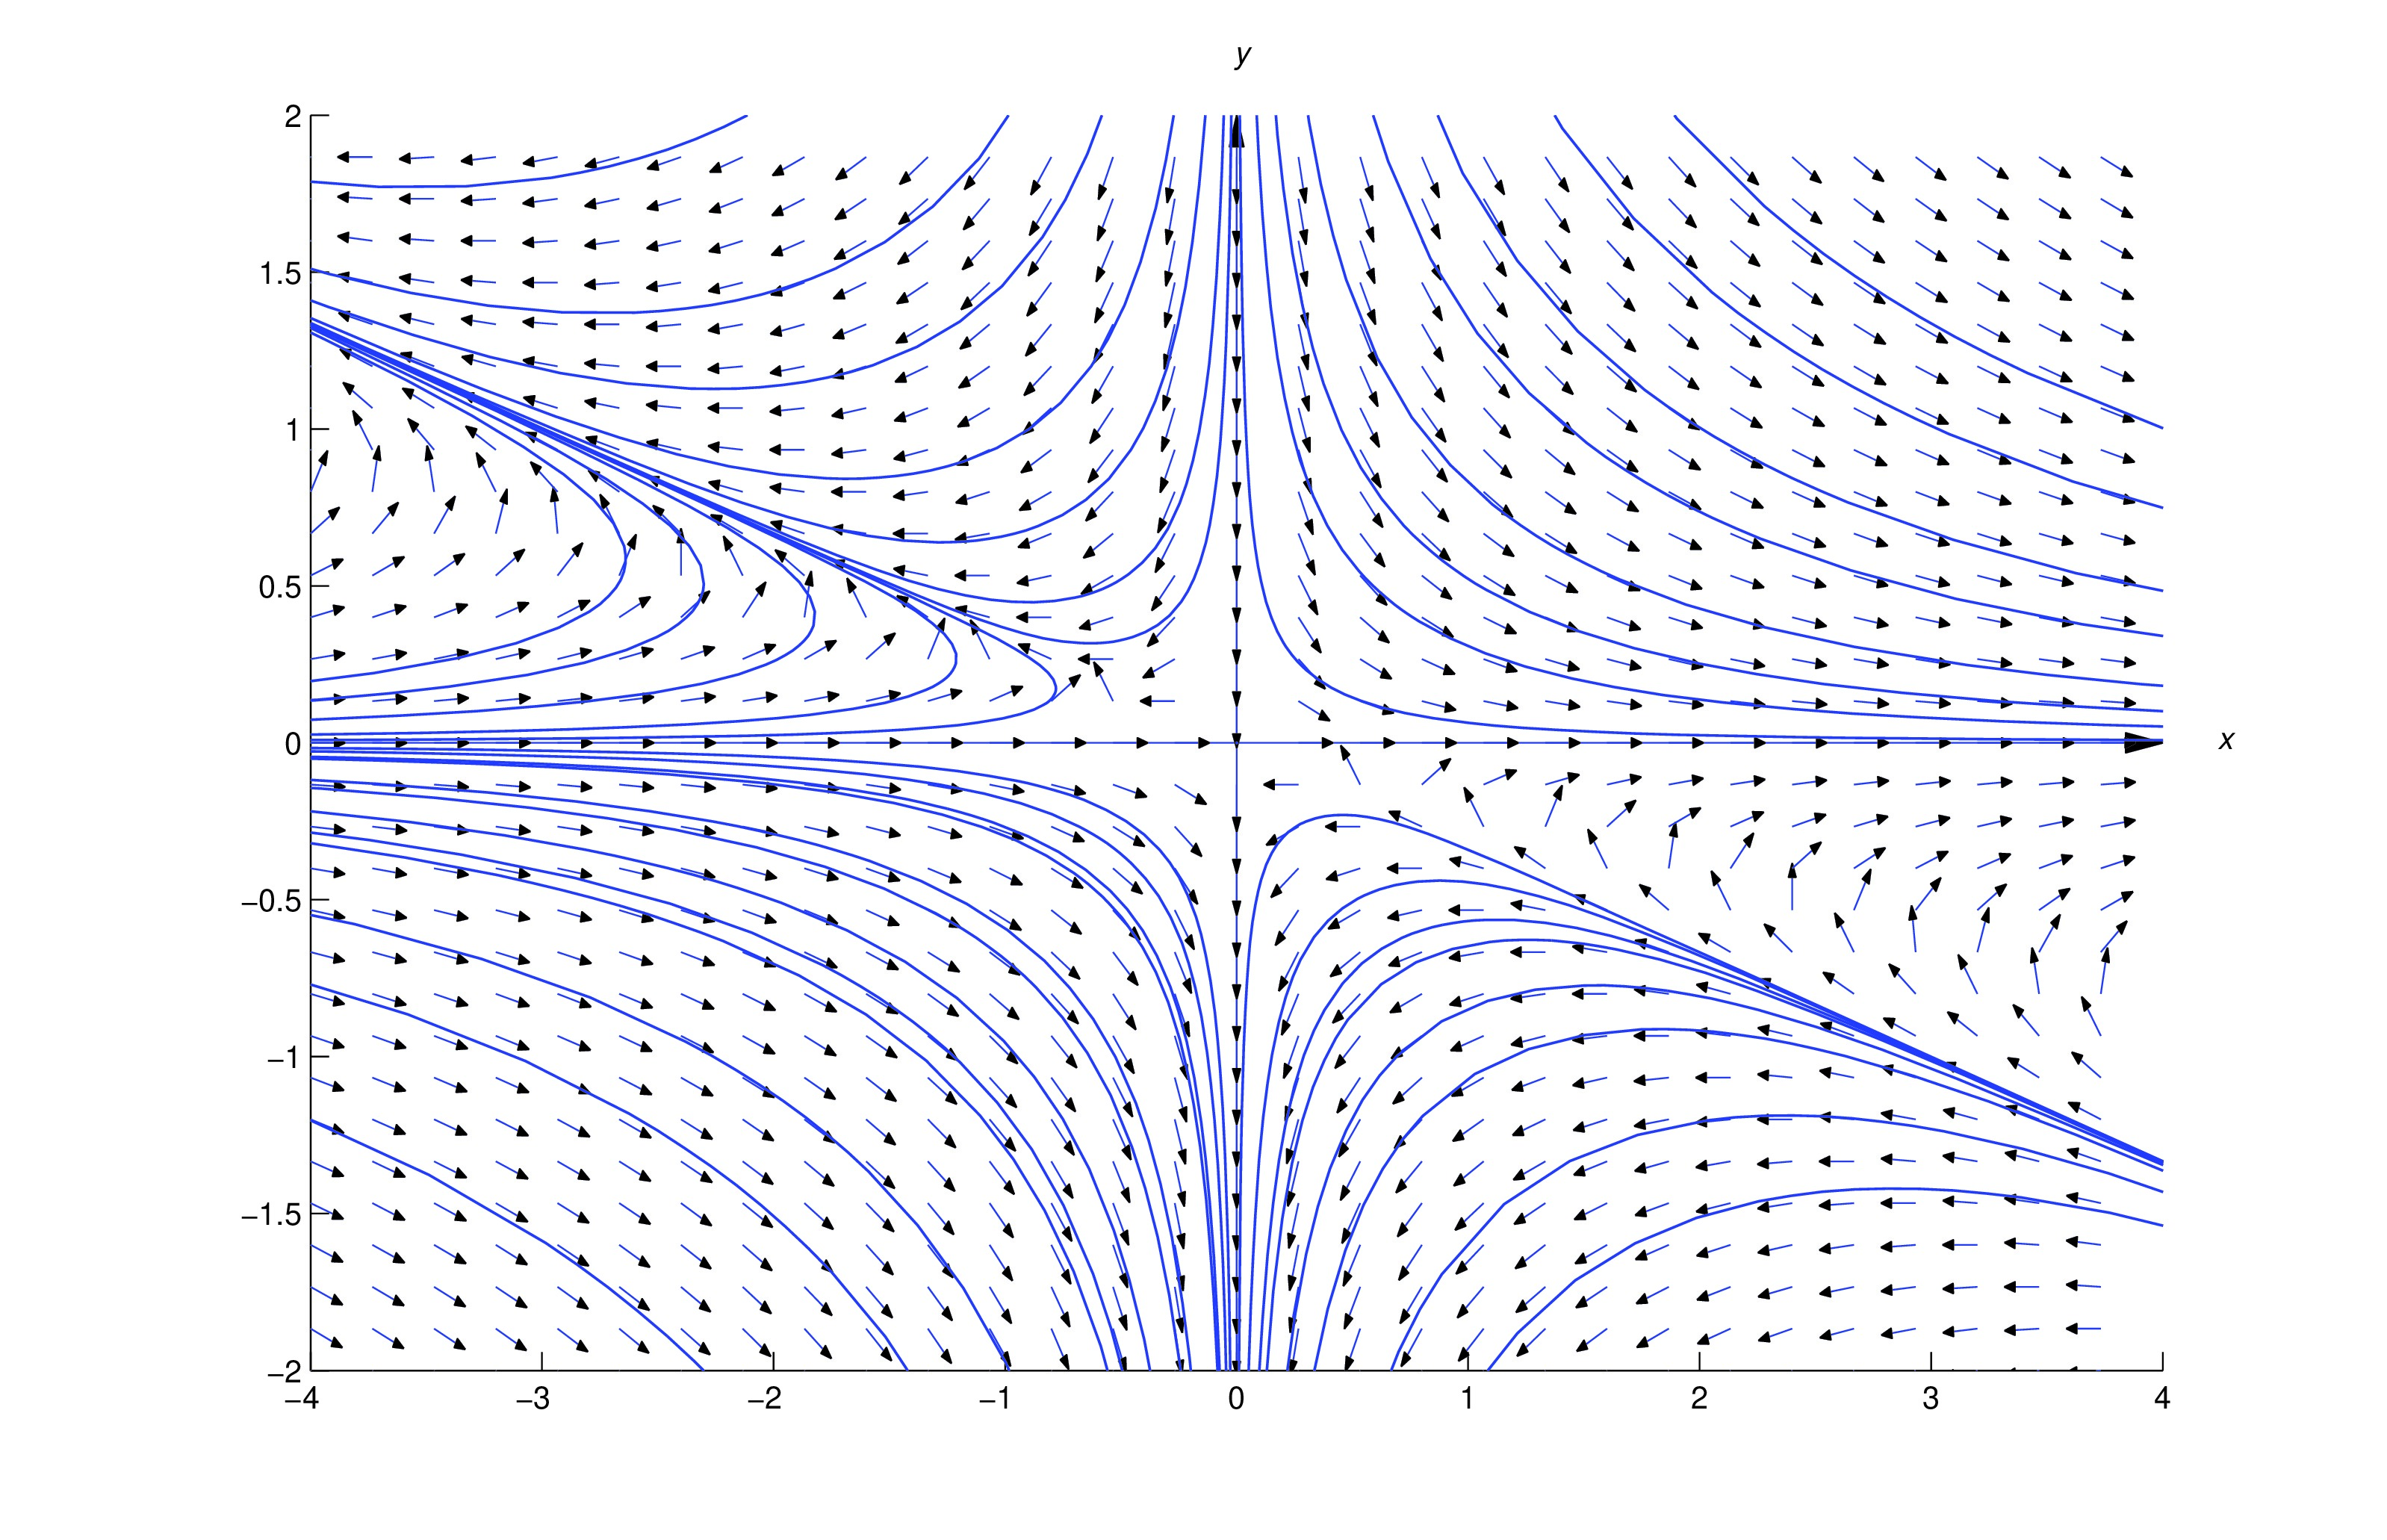
\includegraphics[height=1.5in]{fig020603.jpg}
\end{image}

\end{explanation}
\end{example}


\begin{example}\label{example:2.6.4}
The separable  equation
\begin{equation}\label{eq:2.6.26}
-y\,dx+(x+x^6)\,dy=0
\end{equation}
can be converted to the exact equation
\begin{equation} \label{eq:2.6.27}
-\frac{dx}{x+x^6}+\frac{dy}{y}=0
\end{equation}
by multiplying through
by the  integrating factor
$$
\mu(x,y)=\frac{1}{y(x+x^6)}.
$$
However, to solve \eqref{eq:2.6.27} by the method of \href{https://ximera.osu.edu/ode/main/exactEquations/exactEquations}{Trench 2.5}
we would have to evaluate the nasty integral
$$
\int \frac{dx}{x+x^6}.
$$
Instead, we solve \eqref{eq:2.6.26} explicitly for $y$ by finding  an
integrating factor of the form
$\mu(x,y)=x^ay^b$.

In \eqref{eq:2.6.26}
$$
M=-y, N=x+x^6,
$$
and
$$
M_y-N_x=-1-(1+6x^5)=-2-6x^5.
$$
We  look for functions
$p=p(x)$ and $q=q(y)$ such that
$$
M_y-N_x=p(x)N-q(y)M;
$$
that is,
\begin{equation}\label{eq:2.6.28}
-2-6x^5=p(x)(x+x^6)+q(y)y.
\end{equation}
The right side will contain the term $-6x^5$ if $p(x)=-6/x$.   Then
\eqref{eq:2.6.28} becomes
$$
-2-6x^5=-6-6x^5+q(y)y,
$$
so  $q(y)=4/y$.  Since
$$
\int p(x)\,dx=-\int\frac{6}{x}\,dx=-6\ln|x|=\ln\frac{1}{x^6},
$$
 and
$$
\int q(y)\,dy=\int\frac{4}{y}\,dy=4\ln
|y|=\ln{y^4},
$$
we can take $P(x)=x^{-6}$ and $Q(y)=y^4$,
which yields the integrating factor $\mu(x,y)=x^{-6}y^4$.
Multiplying \eqref{eq:2.6.26} by  $\mu$ yields the exact equation
$$
-\frac{y^5}{x^6}\,dx+\left(\frac{y^4}{x^5}+y^4\right)
\,dy=0.
$$
 We leave it to you to 
show that this equation has the implicit solution 
$$
\left(\frac{y}{x}\right)^5+y^5=k.
$$
 Solving for $y$ yields
$$
y=k^{1/5}x(1+x^5)^{-1/5},
$$
which we rewrite as
$$
y=cx(1+x^5)^{-1/5}
$$
by renaming the arbitrary constant.
 This is also a solution of \eqref{eq:2.6.26}.

The figure below shows a direction field and some integral curves
 for \eqref{eq:2.6.26}.
 
 \begin{image}
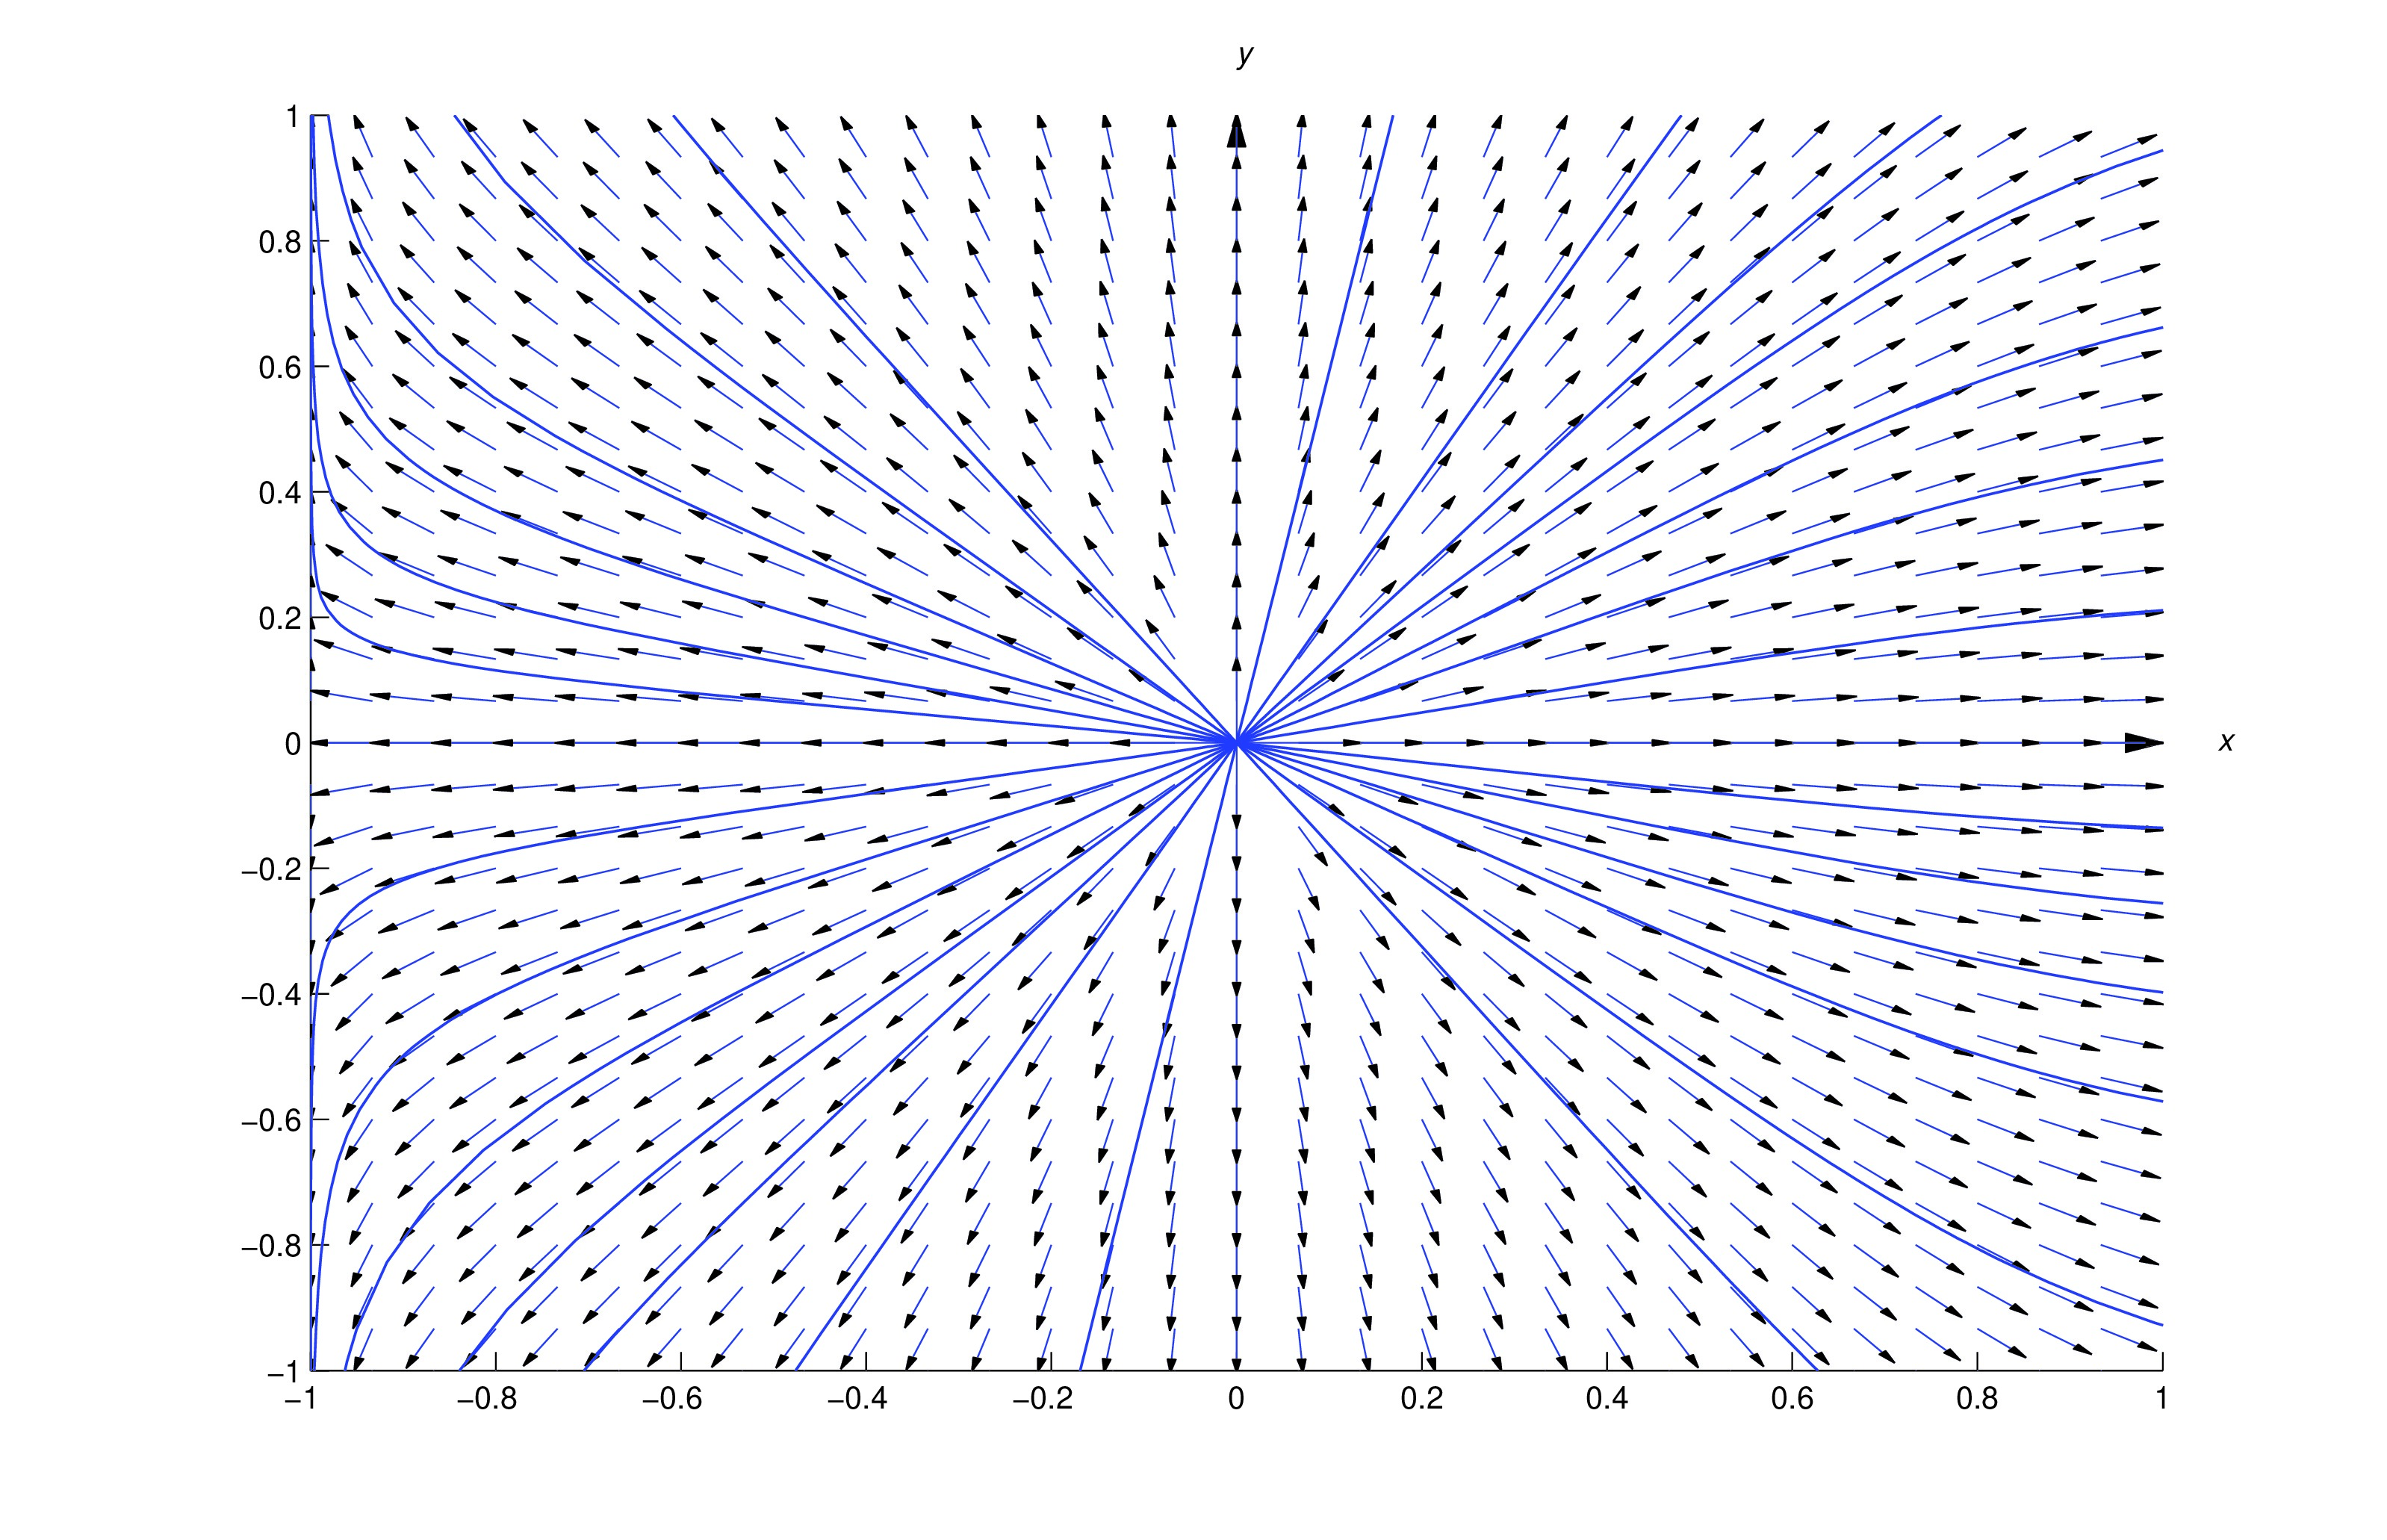
\includegraphics[height=3.66in]{fig020604.jpg}
\end{image}

\end{example}

\section*{Text Source}
Trench, William F., "Elementary Differential Equations" (2013). Faculty Authored and Edited Books \& CDs. 8. (CC-BY-NC-SA)

\href{https://digitalcommons.trinity.edu/mono/8/}{https://digitalcommons.trinity.edu/mono/8/}


\end{document}


